\documentclass{article}

%opening
\title{Simulating Different Receivers in a \\Rayleigh Fading, SISO Environment\\
\large Project \#1}
\author{Intelligent Communication Systems (ICS) Lab.\\노용재}
\date{Winter Intern Seminar (2023-1)}

\usepackage{kotex} % korean
\usepackage[margin=1in]{geometry} % 둘레 margin
\usepackage{matlab-prettifier}
\usepackage{amsmath}
\usepackage{graphicx} % image
\usepackage{subcaption} % subfigure
\usepackage{xcolor} % for coloring text
\usepackage{amssymb} % because, therefore symbol

\newcommand{\bd}{\textbf} % bold
\providecommand{\abs}[1]{\lvert#1\rvert}
\graphicspath{{./img/}}
\newcommand{\sgn}{\operatorname{sgn}}
\begin{document}

\maketitle
\tableofcontents
\vspace{0.5cm}
\hrule
\vspace{0.5cm}

Binary Modulation, 4-QAM, 16-QAM의 modulation 환경에서 Zero-forcing (ZF) receiver, Minimum Mean Square Error (MMSE) receiver, Maximum Likelihood Detection (MLD)의 BER (bit error rate)를 구하기 위해 실험을 MATLAB에서 수행하였다. 실험의 공통된 조건은 다음과 같다.

\begin{itemize}
  \item Es/N0는 -2dB~20dB(2dB 간격)
  \item 신호의 평균전력은 1W이 되도록한다. ($Es=1$)
  \item SISO; Single Input, Single Output
\end{itemize}
\section{Implementation}
$M=2^2n$ $(n=1,2,3,...)$의 상황을 가정하였다.
\subsection{Common Environment Variables}
\begin{equation}
y=hs+n
\end{equation}
\begin{lstlisting}[style=Matlab-editor, frame=single, numbers=left,]
EsN0_dB = -2:2:20;
EsN0 = db2pow(EsN0_dB);

EbN0 = EsN0 / log2(M);
EbN0_dB = pow2db(EbN0);

LengthBitSequence = NumberOfSignals*log2(M); % log2(M) bits per signal

% Bit Generation
BitSequence = randi([0 1], 1, LengthBitSequence);
SymbolSequence = qammod(BitSequence.', M, 'InputType', 'bit', 'UnitAveragePower', 1).';

% Noise (n) Generation
NoiseSequence = (randn(1, length(SymbolSequence)) + 1j * randn(1, length(SymbolSequence))) / sqrt(2); 

% Channel (h) Generation
H = (randn(1, length(SymbolSequence)) + 1j * randn(1, length(SymbolSequence))) ./ sqrt(2);

% Received Signal (y = s + n) Generation
ReceivedSymbolSequence = H .* SymbolSequence + NoiseSequence * sqrt(1 / EsN0(indx_EbN0));

\end{lstlisting}
\subsection{ZF(Zero-forcing)}
\begin{gather}
z=wy : w_{ZF}=(h)^{-1}\\
\hat{s}=\operatorname*{argmin}_s \abs{z-s}^2
\end{gather}
\begin{lstlisting}[style=Matlab-editor, frame=single, numbers=left,]
w_zf = H.^(-1);
DetectionSymbolSequence_ZF = ReceivedSymbolSequence .* w_zf; % Detection (Zero-Forcing: y / h)

DetectionBitSequence_ZF = qamdemod(DetectionSymbolSequence_ZF.', M, 'OutputType', 'bit', 'UnitAveragePower', 1)';
\end{lstlisting}
\subsection{MMSE(Minimum Mean Square Error)}
\begin{gather}
z=wy : w_{MMSE}=(\abs{h}^2+1/\rho)^{-1}h^*\\
\hat{s}=\operatorname*{argmin}_s \abs{z-s}^2
\end{gather}
\begin{lstlisting}[style=Matlab-editor, frame=single, numbers=left,]
w_mmse = (abs(H).^2+1/EsN0(indx_EbN0)).^(-1) .* conj(H);
DetectionSymbolSequence_MMSE = ReceivedSymbolSequence .* w_mmse;
DetectionBitSequence_MMSE = qamdemod(DetectionSymbolSequence_MMSE.', M, 'OutputType', 'bit', 'UnitAveragePower', 1)';
\end{lstlisting}
\subsection{MLD(Maximum Likelihood Detection)}
\begin{lstlisting}[style=Matlab-editor, frame=single, numbers=left,]
alphabet = qammod([0:M-1], M, 'UnitAveragePower', true);
arg = (ones(length(alphabet),1) * ReceivedSymbolSequence) - (alphabet.' * H);
arg = abs(arg).^2;
[val,idx] = min(arg);
DetectionBitSequence_MLD = reshape(de2bi(idx-1, log2(M), 'left-msb')', 1, []);
\end{lstlisting}
\section{결과 및 분석}
\subsection{Normalization Factor}
코드 내에서 직접적으로 쓰이지는 않았지만 생각해볼 만한 부분은 \textsl{Normalization Factor}이다. 이 \textsl{Normalization Factor}를 사용하여 평균 전력이 1W가 되게끔 할 수 있다.\\
\\
\bd{Code1}
\begin{lstlisting}[style=Matlab-editor, frame=single]
alphabet = qammod([0:M-1], M, 'UnitAveragePower', true);
\end{lstlisting}
\vspace{0.1cm}
\bd{Code 2}
\begin{lstlisting}[style=Matlab-editor, frame=single]
Normalization_Factor = sqrt(2/3*(M-1));
alphabet = qammod([0:M-1], M) / Normalization_Factor;
\end{lstlisting}
위의 \textsl{Code 1}과 \textsl{Code 2}는 동일한 결과를 이룬다.\\

$M=2^2n$ $(n=1,2,3,...)$일 때의 \textsl{Normalization Factor}를 일반화 시켜보겠다.\\
일반적인 QAM의 Constellation Diagram을 살펴보면 실수 $\sqrt{M}$개, 허수 $\sqrt{M}$개의 point를 갖는 것을 알 수 있다.\\
하나의 신호에 대한 값을 그 신호의 \textsl{alphabet}이라고하자. $M$개의 \textsl{alphabet}이 다음과 같다고하자.
\begin{equation}
alphabet={\pm(2n-1)\pm j\cdot(2n-1)} \qquad n\in{1,2,...,\frac{\sqrt{M}}{2}}
\end{equation}
그렇다면 신호의 평균전력은 다음과 같이 일반화 가능하다.
\begin{equation}
\begin{split}
E_s=E[\abs{s}^2]&=\frac{1}{M}\sum_{n=1}^M \abs{s_n}^2\\
&=\frac{1}{M}\cdot4\sum_{n=1}^{\frac{\sqrt{M}}{2}} \sum_{m=1}^{\frac{\sqrt{M}}{2}} [(2n-1)^2+(2m-1)^2]\\
&=\frac{1}{M}\cdot4\sum_{n=1}^{\frac{\sqrt{M}}{2}} \sum_{m=1}^{\frac{\sqrt{M}}{2}} [(2n-1)^2] + \sum_{n=1}^{\frac{\sqrt{M}}{2}} \sum_{m=1}^{\frac{\sqrt{M}}{2}}[(2m-1)]^2\\
&=\frac{1}{M}\cdot4\sum_{n=1}^{\frac{\sqrt{M}}{2}} \sum_{m=1}^{\frac{\sqrt{M}}{2}} [(2n-1)^2]\cdot2\\
&=\frac{1}{M}\cdot4\sum_{n=1}^\frac{\sqrt{M}}{2}[(2n-1)^2\cdot\sqrt{M}]\\
&=\frac{4}{\sqrt{M}}\sum_{n=1}^\frac{\sqrt{M}}{2}[4n^2-4n+1]\\
&=\frac{2}{3}(M-1)
\end{split}
\end{equation}
(2)에서의 결과를 토대로 normalization이 이뤄진 alphabet을 구할 수 있다.
\begin{equation}
normalized\ alphabet=\Big{[}\pm\frac{2n-1}{\sqrt{\frac{2}{3}(M-1)}}\pm j\cdot\frac{2n-1}{\sqrt{\frac{2}{3}(M-1)}}\Big{]} \qquad n\in\{1,2,...,\sqrt{M}\}
\end{equation}
해당 결과를 토대로 다시 평균 전력을 구한다면 $E_s$가 1W임을 확인할 수 있다.\\
\\
%\textit{참고자료}\\
\bd{참고자료}\\
다음은 16-QAM의 Constellation이다.\\
\begin{figure}[!ht]
	\centering
	\begin{subfigure}{0.5\textwidth}
		\centerline{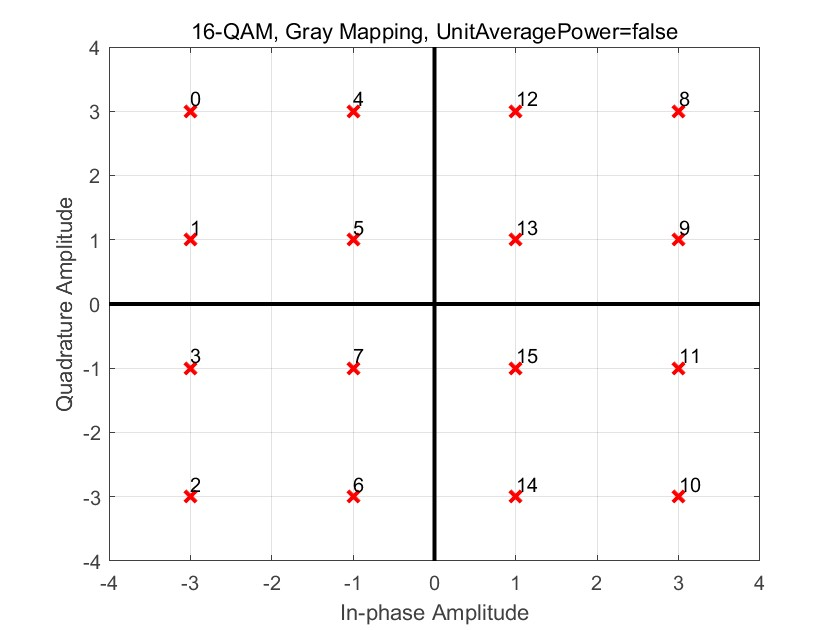
\includegraphics[width=0.8\textwidth]{16qamnonunit.jpg}}
		\caption{Non-normalized Constellation}
	\end{subfigure}%
	\begin{subfigure}{0.5\textwidth}
		\centerline{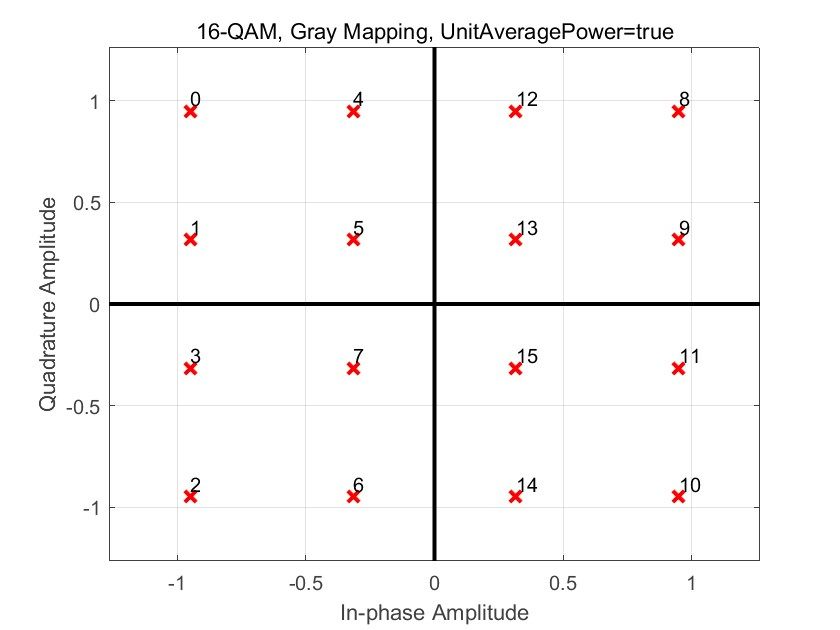
\includegraphics[width=0.8\textwidth]{16qamunit.jpg}}
		\caption{Normalized Constellation}
	\end{subfigure}
	\caption{16-QAM Constellation}
\end{figure}
\\
\subsection{M=2,4일 때 ZF, MMSE, MLD의 BER의 동일성}
실험 결과에 따르면, Binary Modulation일 때와 4-QAM일 때 어떤 ZF, MMSE, MLD 방식을 사용한지와 무관하게 BER이 동일한 것을 관찰할 수 있었다.\\
ZF와 MMSE의 경우를 먼저 살펴보자. ZF와 MMSE에 해당하는 조건식들은 다음과 같다.
\begin{gather}
\hat{s}=\operatorname*{argmin}_s \abs{z-s}^2\\
z=w(hs+n)\\
w_{ZF}=(h)^{-1}\\
w_{MMSE}=(\abs{h}^2+1/\rho)^{-1}h^*
\end{gather}
$z$는 post-processing signal에 해당된다. ZF와 MMSE, 각각의 post-processing signal을 살펴보겠다.\\
\\
\bd{ZF의 Post-processing Signal}
\begin{equation}
\begin{split}
z_{ZF}&=w_{ZF}(hs+n)\\
&=h^(-1)(hs+n)\\
&=s+\frac{n}{h}
\end{split}
\end{equation}
\bd{MMSE의 Post-processing Signal}
\begin{equation}
\begin{split}
z_{MMSE}&=w_{MMSE}(hs+n)\\
&=(\abs{h}^2+1/\rho)^{-1}h^*(hs+n)\\
&=(\abs{h}^2+1/\rho)^{-1}h^*\, h(s+\frac{n}{h})\\
\end{split}
\end{equation}
위의 결과를 토대로 다음과 같이 표현이 가능하다.
\begin{equation}
\begin{split}
z_{MMSE}&=(\abs{h}^2+1/\rho)^{-1}h^*\,h\cdot z_{ZF}\\
\sgn(z_{MMSE}) &= \sgn((\abs{h}^2+1/\rho)^{-1}h^*\,h\cdot z_{ZF})\\
&=\sgn(z_{ZF})\quad (\because (\abs{h}^2+1/\rho)^{-1}h^*\,h \geq 0) \\
\end{split}
\end{equation}
$\sgn(z_{MMSE})=\sgn(z_{ZF})$라는 것은 극 좌표계로 나타냈을 때의 각도가 같다는 것을 의미한다. 이는 amplitude보다는 phase에 영향을 받는 binary modulation이나 4-QAM의 경우, 같은 $h$, $\rho$, $s$의 값이 주어졌을 때 감지되는 signal은 ZF, MMSE 종류와 관계없이 동일해지는 결과를 야기한다.\\
\begin{figure}[!ht]
	\centering
	\begin{subfigure}{0.5\textwidth}
		\centerline{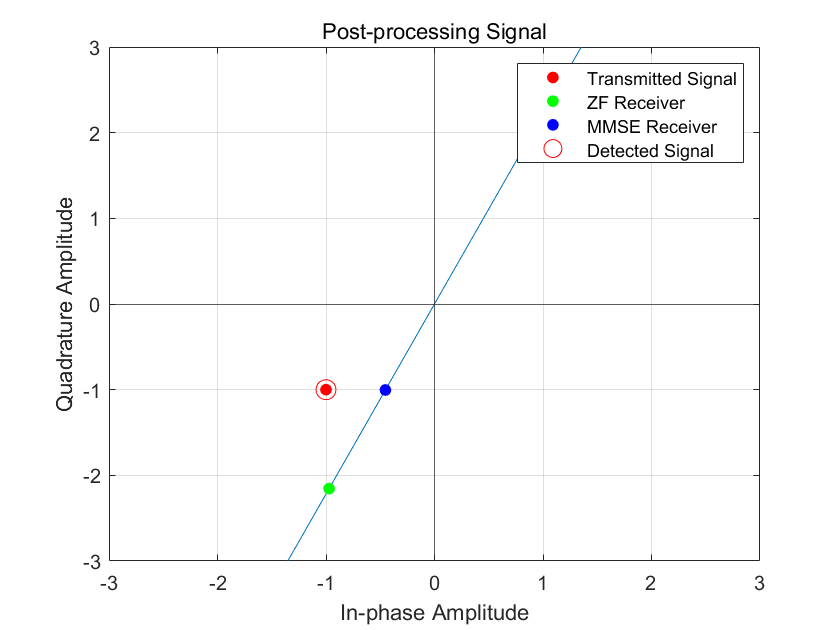
\includegraphics[width=0.8\textwidth]{4qam_correct.png}}
		\caption{Correct Detection Example}
	\end{subfigure}%
	\begin{subfigure}{0.5\textwidth}
		\centerline{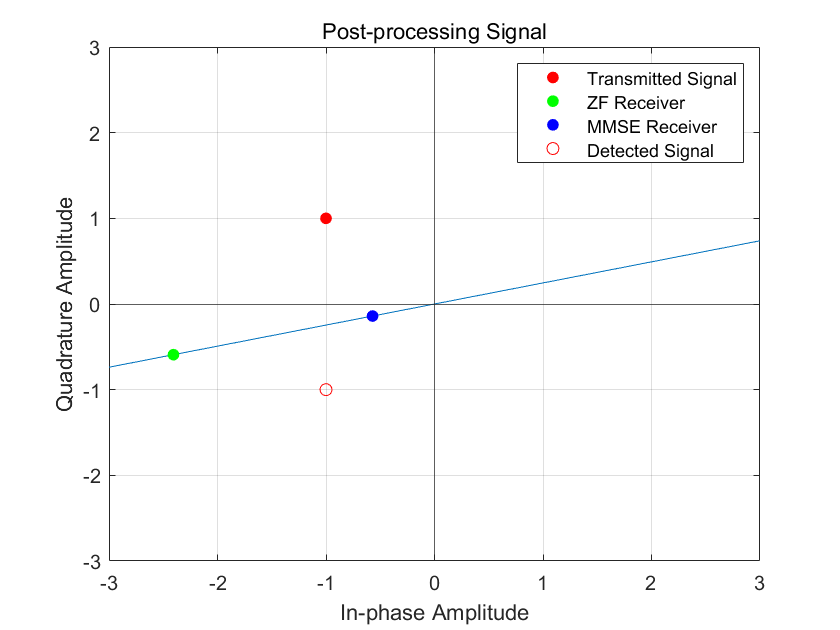
\includegraphics[width=0.8\textwidth]{4qam_error.png}}
		\caption{Signal Detection Error Example}
	\end{subfigure}
	\caption{4-QAM의 ZF, MMSE Post-processing Signal Example}
\end{figure}

\bd{Figure 3}는 \textsl{Matlab}을 통해 $z_{MMSE}$와 $z_{ZF}$를 직교좌표계로 바꾼 뒤, 두 $\theta$ 값을 비교한 것이다. $\theta$값의 차이 중 가장 큰 값은 4.4409$e^{-16}$이었다. 이는 매우 작은 값으로 컴퓨터가 가지는 'finite precision'로 인해 생겨난 오차로 생각할 수 있다. 그러므로 모든 경우에 대해서 $\theta_{MMSE}-\theta_{ZF}=0$가 나타났다고 생각할 수 있다. \bd{Figure 2}의 \textsl{ZF Receiver}와 \textsl{MMSE Receiver}가 하나의 직선 위에 나타난 것을 통해 이를 시각적으로도 확인할 수 있다.
\begin{figure}[h]
	\centering
	\fbox{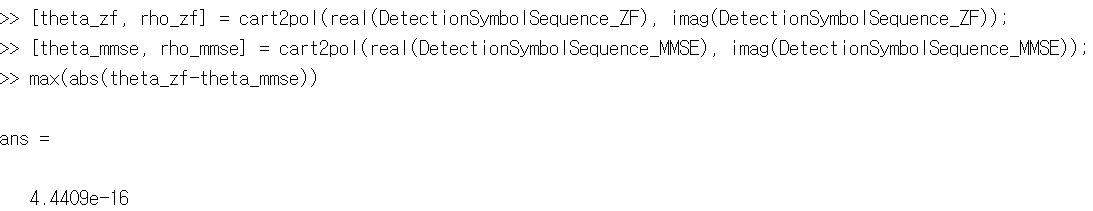
\includegraphics[width=\textwidth]{theta.png}}
	\caption{EsN0=5dB}
\end{figure}
\section{과제 외적 의문점 및 질문}
\begin{itemize}
  \item SNR이 얼마나 커져야 \bd{ZF}와 \bd{MMSE}의 \textsl{BER}이 같아질까? 수학적 공식으로 나타낼 수 있는가?
\end{itemize}
\section{Entire Code}
\begin{lstlisting}[style=Matlab-editor, frame=single, numbers=left,]
close all
clear
clc

% Simulation
M = 16
Nt = 1;
NumberOfSignals = 10^2;
LengthBitSequence = Nt * NumberOfSignals*log2(M); % log2(M) bits per signal

NumberIteration = 10^3;

Es = 1;

EsN0_dB = -2:2:20;
EsN0 = db2pow(EsN0_dB);

EbN0 = EsN0 / log2(M);
EbN0_dB = pow2db(EbN0);

ErrorCount_ZF = zeros(1, length(EbN0_dB));
ErrorCount_MMSE = zeros(1, length(EbN0_dB));
ErrorCount_MLD = zeros(1, length(EbN0_dB));

alphabet = qammod([0:M-1], M, 'UnitAveragePower', true);

for iTotal = 1 : NumberIteration
    BitSequence = randi([0 1], 1, LengthBitSequence); % Bit Generation (BitSequence = rand(1, LengthBitSequence) > 0.5;)
    SymbolSequence = qammod(BitSequence.', M, 'InputType', 'bit', 'UnitAveragePower', 1).';
    %avgPower = mean(abs(SymbolSequence).^2)
    NoiseSequence = (randn(1, length(SymbolSequence)) + 1j * randn(1, length(SymbolSequence))) / sqrt(2); % Noise (n) Generation
    H = (randn(1, length(SymbolSequence)) + 1j * randn(1, length(SymbolSequence))) ./ sqrt(2); % Channel (h) Generation
    for indx_EbN0 = 1 : length(EbN0)
        ReceivedSymbolSequence = H .* SymbolSequence + NoiseSequence * sqrt(1 / EsN0(indx_EbN0)); % Received Signal (y = s + n) Generation

        % ZF Receiver
        w_zf = H.^(-1);
        DetectionSymbolSequence_ZF = ReceivedSymbolSequence .* w_zf; % Detection (Zero-Forcing: y / h)

        % MMSE Receiver
        w_mmse = (H.*conj(H)+1/EsN0(indx_EbN0)).^(-1) .* conj(H);
        z = ReceivedSymbolSequence .* w_mmse;
        arg = (ones(length(alphabet),1) * z) - (alphabet.' * H .* w_mmse);
        arg = arg .* conj(arg);
        [val,idx] = min(arg);
        DetectionSymbolSequence_MMSE = alphabet(idx); % TODO: could possibly simplify it more
        DetectionSymbolSequence_MMSE = z;
        
        % MLD Receiver;
        arg = (ones(length(alphabet),1) * ReceivedSymbolSequence) - (alphabet.' * H);
        arg = abs(arg).^2;
        [val,idx] = min(arg);
        DetectionSymbolSequence_MLD = alphabet(idx);

        % Symbol Sequence -> Bit Sequence
        DetectionBitSequence_ZF = qamdemod(DetectionSymbolSequence_ZF.', M, 'OutputType', 'bit', 'UnitAveragePower', 1)'; % Detection
        DetectionBitSequence_MMSE = qamdemod(DetectionSymbolSequence_MMSE.', M, 'OutputType', 'bit', 'UnitAveragePower', 1)'; % tmp value;
        DetectionBitSequence_MLD = qamdemod(DetectionSymbolSequence_MLD.', M, 'OutputType', 'bit', 'UnitAveragePower', 1)';

        ErrorCount_ZF(1, indx_EbN0) = ErrorCount_ZF(1, indx_EbN0) + sum(DetectionBitSequence_ZF~=BitSequence);
        ErrorCount_MMSE(1, indx_EbN0) = ErrorCount_MMSE(1, indx_EbN0) + sum(DetectionBitSequence_MMSE~=BitSequence);
        ErrorCount_MLD(1, indx_EbN0) = ErrorCount_MLD(1, indx_EbN0) + sum(DetectionBitSequence_MLD~=BitSequence);
    end
%     toc
    
end

BER_Simulation_ZF = ErrorCount_ZF / (LengthBitSequence * NumberIteration);
BER_Simulation_MMSE = ErrorCount_MMSE / (LengthBitSequence * NumberIteration);
BER_Simulation_MLD = ErrorCount_MLD / (LengthBitSequence * NumberIteration);

if M==2
    BER_Theory = berfading(EbN0_dB, 'psk', 2, 1);
else
    BER_Theory = berfading(EbN0_dB, 'qam', M, 1); % not sure if 'dataenc' needs to be specified; I don't even know what it does
end

% Plot
figure()
semilogy(EsN0_dB, BER_Theory, 'r--');
hold on
semilogy(EsN0_dB, BER_Simulation_ZF, 'bo');
semilogy(EsN0_dB, BER_Simulation_MMSE, 'bx');
semilogy(EsN0_dB, BER_Simulation_MLD, 'b^');


axis([-2 20 10^-3 0.5])
grid on
legend('Theory (Rayleigh)', 'ZF (Rayleigh)', 'MMSE (Rayleigh)', 'MLD (Rayleigh)');
xlabel('Es/No [dB]');
ylabel('BER');
title('BER for QAM (M='+string(M)+')');
\end{lstlisting}
\end{document}